\documentclass[pdf]{beamer}
\mode<presentation>{}

\usepackage[utf8]{inputenc}
\usepackage[english,serbian]{babel}

\usetheme{Madrid}
\useoutertheme{miniframes}
\useinnertheme{circles}


\title{Etika u računarstvu}
\subtitle{Seminarski rad}% u okviru kursa\\Metodologija stručnog i naučnog rada\\ Matematički fakultet}
\author[]{Marina Borozan, Matija Miličević,\\
	Stefan Mirić, Nikola Vuković\\}

\begin{document}

\begin{frame}
	\titlepage
	\end{frame}


\begin{frame}
\frametitle{Uvod}

\begin{itemize}
\item{Tehnološki razvoj i nove mogućnosti}
\item{Ubrzane promene u računarstvu}
\item{Moralne dileme i prihvatanje odgovornosti}
\item{Kratak sadržaj:}
	\begin{itemize}
	\item{Uvod u teoriju etike}
	\item{Etika u računarstvu}
	\item{Razvoj tehnologije i primena etike}
	\end{itemize}
\end{itemize}

\end{frame}

\begin{frame}
\frametitle{Etika}

Definicija: Oblast filozofije koja se bavi sistematizacijom, odbranom i preporukom ispravnog i pogrešnog ponašanja.

Podoblasti:
\begin{itemize}
\item{Metaetika

	Bavi se temeljima etike i apstraktnim pitanjima.}
\item{Normativna etika

	Najkorisnija za temu etike u računarstvu. Definiše moralne probleme na praktičan način.}
\item{Primenjena etika
	
	Razmatra konkretne situacije i moralna pitanja. Primenjuje principe definisane u normativnoj etici.}
\end{itemize}

\end{frame}

\begin{frame}
\frametitle{Teorije etike}

\begin{itemize}
\item{Pojam dobrog}
\item{Pojam ispravnog}
\end{itemize}

%TODO ovde tabela podele

\begin{table}
\begin{center}
\begin{tabular}{|l|c|c|c|} \hline
Teorija & Etika vrline & Deontologija & Konsekvencijalizam\\ \hline
Fokus & Delatnik & Delo & Posledice\\ \hline
Predstavnik & Aristotel & Imanuel Kant & Džon Stjuart Mil\\
& 384-322 PNE & 1724-1804 & 1806-1873\\ 
& 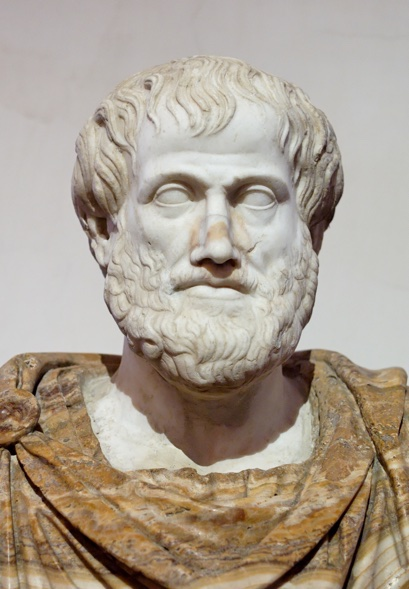
\includegraphics[scale=.1]{slike/aristotel.jpg} & 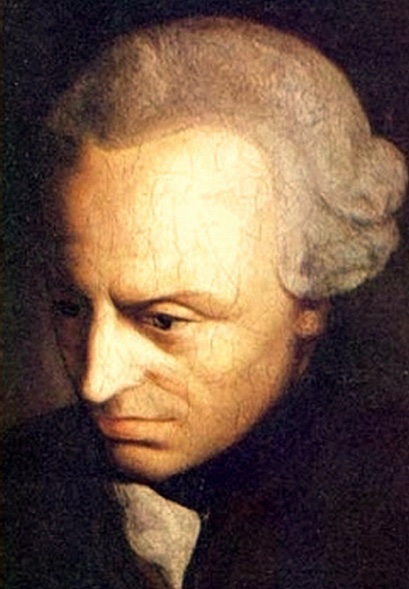
\includegraphics[scale=.1]{slike/kant.jpg} & 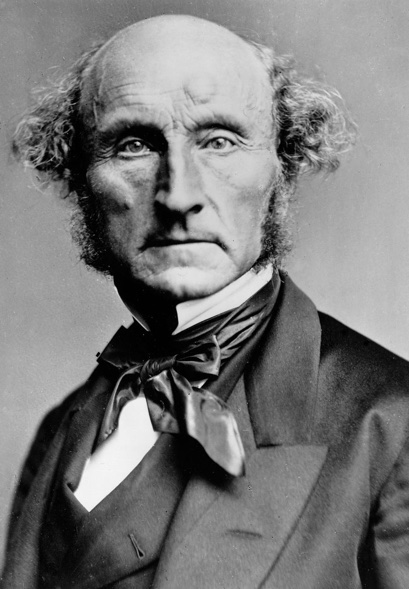
\includegraphics[scale=.1]{slike/mil.jpg} \\
\hline
\end{tabular}
\end{center}
\end{table}


\end{frame}

\begin{frame}
\frametitle{Deontologija}

Naziv potiče od grčkih reči koje označavaju dužnost (deon) i nauku (logos). Procenjuje moralnost postupaka.

%TODO ovde slika Kanta

Kantijanizam - najpoznatija podgrana deontologije.

Principi:
\begin{itemize}
\item{Univerzalnost moralnih zakona}
\item{Dobra volja kao motiv}
\item{Pojam dužnosti} %TODO nalgasiti možda dužnost bojom?
\item{Kategorički imperativ}
\end{itemize}

\end{frame}


\begin{frame}
\frametitle{Etika i tehnološki razvoj}

	Nove tehnologije:

	\begin{itemize}

	\item Nove mogućnosti

	\item Novi problemi

	\end{itemize}

%\pause
	Stavovi o tehnološkom napretku:

	\begin{enumerate}

	\item Tehnicizam %TODO Dodati kratak opis.
	\item Optimizam
	\item Skepticizam

	\end{enumerate}

	\end{frame}


\begin{frame}
\frametitle{Računarska Etika}
	%Pričati o tome šta je računarska etika u sklopu priče o istoriji.
	
	Kratka istorija:
	\begin{itemize}
	
	\item Norbert Viner
	\begin{itemize}
	\item[--] ``Kibernetika'' (1948) %TODO Reference! Tačka iza godine?
	\item[--] ``Ljudska upotreba ljudskih bića'' (1950)
	\end{itemize}
	
	\item Volter Maner
	\begin{itemize}
	\item[--] Eksperimentalni kurs (1976)
	\item[--] Plan kursa (1978)	
	\item[--] Monograf (1980) %TODO Saznaj šta je monograf.
	\end{itemize}
	\end{itemize}
	\end{frame}

\begin{frame}
\frametitle{Viđenja Računarske Etike}

	Pristupi u naučnoj literaturi: %Da li je ok ovo italik? Da li treba eng.?
	\begin{enumerate}
	\item Pristup nepostojanja (\textit{No resolution approach})
	\item Profesionalni pristup (\textit{The professional approach})
	\item Radikalni pristup (\textit{The radical approach})
	\item Konzervativni pristup (\textit{The conservative approach})
	\item Inovativni pristup (\textit{The innovative approach})
	\end{enumerate}
	\end{frame}


\begin{frame}
\frametitle{Primeri etičkih dilema u računarstvu}
		Pisanje virusa:
		\begin{itemize}
		\item Kalgari Univerzitet (Ken Barker)
			\begin{itemize}
			\item Pisanje virusa na kursu računarske sigurnosti
			\item Zabrinutost antivirusnih kompanija 
			\end{itemize}
		
		\item Sonoma Univerzitet (Džordž Ledin)
			\begin{itemize}
			\item Osnovao kurs za pravljenje bolje sigurnosne zaštite
			\item Bojkot sigurnosnih kompanija
			\end{itemize}
		\end{itemize}
\end{frame}


\begin{frame}
\frametitle{Preporuke etičkog postupanja}

	Predlozi institucija:
	\begin{itemize}
		\item Association for Computing Machinery - ACM %u zagradi bolje? (ACM)
		\\- Kodeks etičkog i profesionalnog ponašanja %TODO Sredi + referenca
		\item The Computer Ethics Institute - CEI %(CEI)
		\\- 10 zapovesti računarske etike %TODO referenca
	\end{itemize}


\end{frame}


\begin{frame}
\frametitle{Primeri etičkih dilema u računarstvu}
	Neki dodatni primeri:
	\begin{itemize}
	\item Da li je prihvatljivo da se kupi softver pa onda instalirati ga dvaput?
	\item Šta ako ga instaliramo, a zatim napravimo 50 kopija i prodamo zainteresovanim kupcima?
	\item Da li kompanija ima pravo da čita elektronsku poštu svojih zaposlenih?
	\item Da li kompanija ima pravo da nadzire koje Web stranice njeni zaposleni posećuju?
	\item Da li korisnik ne sme da modifikuje program iako je njegov cilj da ga poboljša?
	%smisliti jos neki primer
	\end{itemize}
\end{frame}

\begin{frame}
\frametitle{Zaključak}
	%TODO (Matija)
	\end{frame}


\begin{frame}
\frametitle{Literatura}
	%TODO
	\end{frame}

\end{document}

